%%%%%%%%%%%%%%%%%%%%%%%%%%%%%%%%%%%%%%%%%%%%%%%%%%%%%%%%%%%%%
%
% Exercises template
%
% Author: Francisco Luque Sánchez (@pacron on github)
%
% Feel free to download, use and share this template :)
%
%%%%%%%%%%%%%%%%%%%%%%%%%%%%%%%%%%%%%%%%%%%%%%%%%%%%%%%%%%%%%


\documentclass[12pt]{article}       % class document and font size
\usepackage[utf8]{inputenc}         % allowance of accents (spanish writing)
\usepackage{indentfirst}

% packages for math fonts
\usepackage{amsmath}
\usepackage{amsfonts}
\usepackage{mathtools}
\usepackage{amsthm}
\newtheorem{theorem}{Teorema}
\newtheorem{lemma}[theorem]{Lema}
\renewenvironment{proof}{{\noindent     \bfseries Demostración}\\}

\usepackage{fancyhdr}               % fancy header: customize your header
\usepackage{geometry}               % set margins in easy way

\geometry{a4paper, margin=1in}      % set 1 inch in every margin

% creation of \qed command to add a black square at the end of line
% \renewcommand*{\qed}{\hfill\ensuremath{\blacksquare}}

% header and footer customisation
\pagestyle{fancy}                   % pagestyle
\fancyhf{}                          % erase previous header and footer content
\rhead{Método de Euler en SED}           % right side of header (Usually document or chapter title)
\lhead{Métodos numéricos II}        % left side of header (Usually name)
\chead{}                            % center of header (useless piece of shit :D)
\rfoot{\thepage}                    % right side of footer (page number)
\lfoot{}                            % left side of footer (empty)
\cfoot{}                            % again a center

% Change the tolerance of hyphenation tool
\pretolerance=2000
\tolerance=3000

%Configuración de tablas
\usepackage{longtable}
\usepackage{rotating}
\usepackage{array}
\usepackage{multicol}
\usepackage{multirow}
\usepackage{booktabs}
\usepackage{float}

% Report title
\title{
    Método de Euler en sistemas de ecuaciones diferenciales \\              % Title
    \large Métodos numéricos II              % Subtitle
}

% Own author header
\author{
        María del Mar Ruiz Martín \\
        Antonio R. Moya Martín-Castaño \\
        Francisco Luque Sánchez \\
        Doble Grado de Ingeniería Informática y Matemáticas\\
        Universidad de Granada - UGR\\
        18001 Granada, \underline{Spain}
}
\date{\today}

\begin{document}
\maketitle

\section{Introducción}

En este trabajo explicaremos el método de Euler para resolución numérica de sistemas de ecuaciones diferenciales de primer orden. Este método es una extensión a sistemas de ecuaciones del método de Euler para ecuaciones diferenciales. Aunque no es muy utilizado en la práctica, ya que por sus características no aporta soluciones lo suficientemente buenas, sí que se suele explicar como introducción a los métodos de resolución numérica de ecuaciones diferenciales, dada su simplicidad. Además, es el más básico de lo que se conocen como \textit{métodos explícitos de resolución numérica de EDs}, y el más básico de los métodos de \textit{Runge-Kutta}. Por tanto, suele ser una buena estrategia introducir este método previo a la explicación de los métodos nombrados, ya que los mismos son una generalización de éste.\\

El trabajo irá estructurado de la siguiente forma. Primero, daremos una descripción general del concepto de sistema de ecuaciones diferenciales, ya que será el objeto sobre el que trabajaremos. Concretamente, nos centraremos en sistemas de ecuaciones diferenciales de primer orden. Tras esto, veremos cómo podemos transformar una ecuación diferencial de orden superior en un sistema de ecuaciones diferenciales de primer orden, con el fin de tratar una ecuación diferencial de orden superior con el método de Euler. Posteriormente, explicaremos el método de Euler y su aplicación a los sistemas de ecuaciones diferenciales. Completaremos este apartado con la resolución de dos ejemplos con este método. Por un lado, resolveremos un sistema de ecuaciones diferenciales de primer orden aplicando el método directamente, y por otro, tomaremos una ecuación de orden superior, la convertiremos en un sistema de ecuaciones, y resolveremos dicho sistema con el método nuevamente.\\

\section{Descripción general de un sistema de ecuaciones diferenciales}

Para comenzar, veamos lo que es una ecuación diferencial. Una ecuación diferencial es una igualdad en la que interviene una variable independiente ($t$), una variable dependiente ($x(t)$) y las sucesivas derivadas de la variable dependiente respecto de la independiente. En forma general, podemos escribir dicha ecuación de la siguiente forma:

$$ F(t, x, x', ..., x^{n)}) = 0 $$

Se define el orden de dicha ecuación diferencial como el mayor orden de derivación de la variable dependiente que aparece en dicha ecuación.\\

Una solución de esta ecuación es un conjunto de funciones que satisfacen las condiciones de dicha ecuación.\\

Asociado a esta ecuación diferencial, se define un problema de valores iniciales (PVI) como dicha ecuación diferencial junto con los $n$ valores siguientes. Fijado $t_0$:

$$ x(t_0) = y_0, x'(t_0) = y_1, ..., x_{n-1}(t_0) = y_{n-1} $$

Se dice que un PVI está bien planteado si existe solución, es única y depende de forma continua de los datos del problema.\\

Pasamos ahora a definir el concepto de sistema de ecuaciones diferenciales. Un sistema de ecuaciones diferenciales es un conjunto de ecuaciones diferenciales en las que se ven implicadas una variable independiente, un conjunto de variables dependientes de la misma, y las sucesivas derivadas de dichas variables dependientes respecto de la independiente. En forma general, podemos escribir un sistema de ecuaciones diferenciales como sigue:

$$
\begin{cases}
F_1(t, x_1, x_1', ..., x_1^{n_1)}, ..., x_m, x_m', ..., x_m^{n_m)}) = 0 \\
F_2(t, x_1, x_1', ..., x_1^{n_1)}, ..., x_m, x_m', ..., x_m^{n_m)}) = 0 \\
\vdots \\
F_r(t, x_1, x_1', ..., x_1^{n_1)}, ..., x_m, x_m', ..., x_m^{n_m)}) = 0
\end{cases}
$$

Al igual que para las ecuaciones diferenciales, la solución de un sistema de ecuaciones diferenciales está compuesto por un conjunto de ecuaciones que satisfacen las condiciones impuestas por las ecuaciones del sistema.\\

De nuevo, podemos definir un PVI asociado al sistema de ecuaciones anterior. Dicho PVI viene definido por el sistema de ecuaciones diferenciales más el siguiente conjunto de valores:
$$ x_1(t_0) = y_{10}, ..., x_1^{n_1-1)}(t_0) = y_{1n_1-1}, ..., x_m(t_0) = y_{m0}, ..., x_1^{n_m-1)}(t_0) = y_{mn_m-1} $$

Se dice que un sistema de ecuaciones diferenciales está bien planteado si cumple las propiedades definidas previamente:

\begin{itemize}
\item $\exists$ solución
\item Es única
\item Depende de forma continua de las propiedades del problema
\end{itemize}

Durante el trabajo, dado que el método de Euler se aplica a ecuaciones y sistemas de primer orden, trabajaremos con este tipo de sistemas. Podemos escribir este tipo de sistemas de la siguiente manera:

$$
\begin{cases}
F_1(t, x_1, ..., x_m) = \frac{d x_1}{d t} \\
F_2(t, x_1, ..., x_m) = \frac{d x_2}{d t} \\
\vdots \\
F_m(t, x_1, ..., x_m) = \frac{d x_m}{d t}
\end{cases}
$$

Y asociado a este sistema de ecuaciones, el PVI definido por el sistema anterior y el conjunto de valores:

$$ x_1(t_0) = y_1, x_2(t_0) = y_2, ..., x_m(t_0) = y_m $$

Notemos también que podemos escribir el sistema anterior haciendo uso de una notación vectorial. De esta forma, tenemos que podemos escribir dicho sistema como sigue:

$$
X'(t)=F(t,X(t)), \, 
X(t)=\begin{bmatrix}
    x_1(t) \\
    \vdots \\
    x_n(t)
    \end{bmatrix}
$$

Diremos que el PVI está bien planteado y satisface las condiciones anteriores. Tenemos una caracterización de problema bien planteado a partir de la condición de Lipschitz. Dado el sistema anterior, diremos que la función vectorial $F(t, X(t))$ satisface la condición de Lipschitz, con constante de Lipschitz $L$, si se cumple que $\forall t_1, t_2 \in [a,b]$ se cumple:

$$ ||F(t_1, X(t_1)) - F(t_2, X(t_2))|| \leq L||X(t_1) - X(t_2)||$$

Tenemos entonces que el problema anterior es un problema bien planteado si $F(t, X(t))$ es continua en su conjunto de definición y Lipschitziana.

\section{Ecuaciones diferenciales de orden superior y reescritura como sistemas}

En la sección anterior definimos el concepto de ecuación diferencial de orden superior y el de sistema de ecuaciones diferenciales. Veamos ahora cómo reescribir una ecuación diferencial de orden $n$ en un sistema de ecuaciones diferenciales en el que se tienen $n$ ecuaciones diferenciales de primer orden. Este paso es necesario para poder aplicar posteriormente el método de Euler, ya que este método sólo puede ser aplicado a ecuaciones diferenciales de primer orden. Veamos entonces esta forma de reescribir las ecuaciones diferenciales de orden superior. Sea la ecuación diferencial de orden $n$: $ F(t, x, x', ..., x^{n)}) = 0 $. Podemos escribir el siguiente sistema de ecuaciones diferenciales, cuya solución es equivalente a la de la ecuación anterior. Tomamos los siguientes cambios de variable:

$$y_0 = x, y_1 = x', y_2 = x'', \dots, y_{n-1} = x^{n-1)}$$

Entonces, la solución de $y_0$ para el siguiente sistema de ecuaciones siguiente es la solución de la ecuación diferencial inicial:

$$
\begin{cases}
y_0' = x' = y_1\\
y_1' = x'' = y_2\\
\vdots\\
y_{n-2}' = x^{n-1)} = y_{n-1}\\
y_{n-1}' = x^{n)} = F(t, y_1, y_2, \dots, y_{n-1})
\end{cases}
$$

Una vez convertida la ecuación en el sistema anterior, estamos en condiciones de aplicar el método de Euler para resolverlo.

\section{Método de Euler para sistemas de ecuaciones diferenciales}

Recordemos primero el método de Euler para un problema de valores iniciales (PVI) bien planteado. Si tomamos puntos en el intervalo [a,b] y un N natural, de forma que $h=(a+b)/N$. Para cada i=0,...,N, los puntos serían
$$ 
t_i=a+ih;
$$
y dado el PVI:
$$
\begin{cases}
y'(t)=f(t,y(t)) \\ 
y(t_0)=y_0
\end{cases}
$$

Podemos tratar de aproximar la solución mediante el método de Euler. Mediante el desarrollo de Taylor centrado en $t_i$ evaluando en el punto $t_{i+1}$:
$$
y(t_{i+1})=y(t_i) + y'(t_i)(t_{i+1}-t_i) + y''(\xi_i)(t_{i+1}-t_i)^2/2
$$

para algún $\xi_i$ entre $(t_i, ti_{i+1})$.

Si observamos, lo escrito anteriormente es equivalente a:
$$
y(t_{i+1})=y(t_i) + f(t_i,y(t_i))h + y''(\xi_i)h^2/2,
$$ 

y lo que es lo mismo:

$$
y(t_{i+1})=y(t_i) + f(t_i,y(t_i))h + O(h^2).
$$

De este modo el método de Euler construye un $w_i \approx y(t_i)$ para cada $i=1,...,N$
$$
\begin{cases}
w_0=y_0\\
w_{i+1}=w_i + hf(t_i,w_i)
\end{cases}
$$

Para el caso de sistemas de ecuaciones diferenciales de primer orden:
$$
\begin{cases}
x_1'=F_1(t,x_1(t),...,x_n(t)) \\
\vdots\\
x_n'=F_n(t,x_1(t),...,x_n(t))
\end{cases}
$$

tenemos que para cada $j=1,...,n$, podemos hacer una aproximación de $w_{i,j} \approx x_j(t_i)$ de forma que:
$$
\begin{cases}
w_{0,j}=x_{j,0} \\
w_{i+1,j}=w_{i,j}+ hF_j(t_i,w_{i,j})
\end{cases}
$$

De este modo, escribiendo el sistema con la siguiente notación matricial:
$$
X'(t)=F(t,X(t))
$$
donde X(t) es de la forma:

\begin{equation*}
X(t)=\begin{bmatrix}
	x_1(t) \\
	\vdots \\
	x_n(t)
	\end{bmatrix}
\end{equation*}
y F(t,X(t)):
\begin{equation*}
F(t,X(t))=\begin{bmatrix}
F_1(t,x_1(t),...,x_n(t)) \\
\vdots \\
F_n(t,x_n(t),...,x_n(t))
\end{bmatrix}
\end{equation*}

podemos expresar una aproximación $W_i \approx X(t_i)$ de a siguiente manera:
$$
\begin{cases}
W_0=X(t_0)\\
W_{i+1}=W_i + hF(t_i,W_i)
\end{cases}
$$
donde $W_i$ es de la forma:

\begin{equation*}
W_i=\begin{bmatrix}
w_1(t_i) \\
\vdots \\
w_n(t_i)
\end{bmatrix}
\end{equation*}

\section{Estudio del error y análisis de la convergencia del método}

\subsection{Análisis de la convergencia}

Para ver la convergencia del método, vamos a definir dos conceptos previos, que son consistencia y estabilidad. El cumplimiento de estas dos propiedades nos asegurará la convergencia del método. Comenzamos definiendo la consistencia de un método. Se dice que un método es consistente si el error de truncamiento que se produce con el método tiende a 0 cuando el tamaño del paso tiende a 0. Es decir, sea $\tau_i(h)$ el error local de truncamiento cometido en el paso $i$, entonces:

$$ \lim_{h \rightarrow 0} max | \tau_i(h) | \rightarrow 0 $$

Veremos más adelante que el método de Euler para sistemas es consistente, cuando hagamos un estudio del error local. Definimos ahora la propiedad de estabilidad. Esta propiedad nos dice cómo se propagan los errores en los datos iniciales al utilizar el algoritmo. Se dice que un método es estable si una perturbación en los datos de entrada no se ve maximizado cuando se utiliza el método para obtener la solución al problema. De forma más rigurosa, se dice que el método es estable si dado un PVI, con $F(t, X(t))$ Lipschitziana, con $X_0$ como valor inicial exacto y $X'_0$ como valor de entrada (con una pequeña perturbación), existe una constante $K$ tal que $|\omega' - \omega| \leq K|X'_0 - X_0|$.\\

Para finalizar, tenemos que por el teorema de Lax-Richtmyer, que no demostraremos por su dificultad, la consistencia y la estabilidad de un método implican su convergencia. Procedemos al estudio del error, que nos dará la consistencia y estabilidad para el método de Euler, por lo que podremos asegurar su convergencia.\\

Antes de comenzar con el estudio del error, comenzaremos definiendo los tipos de errores que se pueden encontrar cuando se utilizan métodos numéricos para resolución de ecuaciones diferenciales:

\begin{description}
\item[Error local] Se define como el error que se produce en un sólo paso del algoritmo, si se supone que el valor obtenido en la aproximación anterior es exacto.
\item[Error global] Se define como el error total cometido con la aproximación tras las $n$ iteraciones del método. Como veremos más adelante, no es la suma de los errores locales cometidos en todas las iteraciones, sino que se ve incrementado.
\item[Error de truncatura] Es el error que se produce por la precisión finita de las máquinas que se utilizan para computar los cálculos.
\end{description}

Estudiemos ahora los errores definidos en el método de Euler aplicado a sistemas de ecuaciones diferenciales.

\subsection{Error local}

Como ya hemos dicho antes, se define el error local como el que se produce en un paso del algoritmo, suponiendo que el valor del que partimos $(t_i, X_i)$ es un valor real del sistema de ecuaciones. Entonces, tenemos que el error local cometido en la iteración $i+1$ lo podemos expresar como $E_{i+1} = ||X(t_{i+1}) - [X(t_{i}) + h*F(t_i, X_i)] ||$. Veamos cómo 

\begin{theorem} Error local del método de Euler.\\

El error local para el método de Euler es $O(h^2)$, donde $h$ es el tamaño del paso que hemos elegido para aplicar el método ($h=(b-a)/N$).

\end{theorem}

\begin{proof}
Veamos la demostración de dicho resultado. Tomamos el PVI asociado al sistema de ecuaciones diferenciales:
$$ X' = F(t, X),\, X(t_0) = X_0 $$
Supongamos que tenemos el valor exacto para un determinado $t_i$, es decir, tenemos $(t_i, X_i)$ exacto. Entonces, el error local para la siguiente iteración es $|| E_{i+1} || = ||X(t_{i+1}) - [X(t_{i}) + h*F(t_i, X_i)] ||$. Tomando cada una de las componentes por separado, y expresando $x_j(t_{i+1}), j = 1, ..., n$ usando su polinomio de Taylor centrado en $t_i$ tenemos:
$$ x_j(t_{i+1}) = x_j(t_i) + h*x'_j(t_i) + \frac{h^2}{2}*x''_j(t_i) + \frac{h^3}{3!}*x'''_j(t_i) + ... = $$
$$ = x_j(t_i) + h*x'_j(t_i) + \frac{h^2}{2}*x''_j(\xi_j) $$
Donde $h = t_{i+1} - t_i$. Con el método de Euler, la aproximación que obtenemos para $x_j(t_i) = \omega_{i+1, j}$ es:
$$ \omega_{i+1, j} = x_j(t_i) + h*f_j(t_i, x_1, ..., x_n) = x_j(t_i) + h*x'_j(t_i) $$
Restando ambas expresiones, tenemos que para cada $x_j$, el error cometido en un paso del método es:
$$ e_{i+1, j} = | x_j(t_{i+1}) - \omega_{i+1, j} | = \frac{h^2}{2}*x''_j(\xi_{i+1, j}),\, \xi_{i+1, j} \in [t_i, t_{i+1}] $$
Tenemos entonces que el vector de los errores lo podemos expresar como sigue:

\begin{equation*}
E_{i+1}=\begin{bmatrix}
e_{i+1, 1} \\
\vdots \\
e_{i+1, n}
\end{bmatrix}=\begin{bmatrix}
\frac{h^2}{2}*x''_1(\xi_{i+1, 1}) \\
\vdots \\
\frac{h^2}{2}*x''_n(\xi_{i+1, n})
\end{bmatrix}
\end{equation*}

Tomando ahora la norma euclídea del vector de los errores, tenemos que el error es $O(h^2)$\\
\qed
\end{proof}

Merece la pena hacer ahora la apreciación de la consistencia del método de Euler. Como acabamos de demostrar, el error local depende de $h^2$, por lo que cuando $h$ tienda a 0, tendremos que el máximo de los errores locales tenderá también a 0, por tanto el método es consistente.\\

Una vez visto el error local que se comete con el método de Euler, pasamos a estudiar el error global que se comete.

\subsection{Error global}

Como ya dijimos en la introducción de este apartado, se define el error global como el error total cometido tras las $n$ iteraciones que se realizan del método. Aunque cabría esperar que el error cometido con el método fuese la suma de los errores que se cometen en cada una de las iteraciones, esto no es cierto. Esto se debe a que, en cada pasa, el error previo cometido se ve levemente incrementado. Pasamos a estudiar entonces dicho error. Necesitaremos de dos lemas previos, que usaremos luego en la demostración:

\begin{lemma}
Para toda $x \geq -1$ y para cualquier $m$ positiva, tenemos que $0 \leq (1 + x)^m \leq e^{mx}$
\end{lemma}

\begin{proof}
Aplicamos el teorema de Taylor a $e^x$. Obtenemos:
$$ e^x = 1 + x + \frac{1}{2}x^2e^\xi $$

donde $0 < \xi < x$. Por tanto:
$$ 0 \leq 1 + x \leq 1 + x + \frac{1}{2}x^2e^\xi = e^x $$ 
y como $1 + x \geq 0$:
$$ 0 \leq (1 + x)^m \leq (e^x)^m = e^{mx} $$
\qed 
\end{proof}

\begin{lemma}
Si $s$ y $t$ son números reales positivos, $\{a_i\}^k_{i=0}$ es una sucesión que satisface $ a_0 \geq -t/s$ y
$$a_{i+1} \leq (1+s)a_i + t, \, \forall i=0, 1, ..., k$$
entonces se tiene que
$$a_{i+1} \leq e^{(i+1)s}\left( a_0 + \frac{t}{s}\right) - \frac{t}{s}$$
\end{lemma}

\begin{proof}
Para un entero fijo $i$, la primera desigualdad del lema implica que:
$$a_{i+1} \leq (1+s)*a_i + t \leq (a+s)[(1+s)a_{i-1} + t] + t \leq ...$$
$$ ... \leq (1+s)^{i+1}a_0 + [1 + (1+s) + ... + (1+s)^i]t $$

Por otro lado, tenemos que $1 + (1+s) + (1+s)^2 + ... + (1+s)^i$ es una serie geométrica de razón $(1+s)$, y que por tanto su suma vale:
$$ \frac{1 - (1+s)^{i+1}}{1 - (1+s)} = \frac{1}{s}[(1+s)^{i+1} - 1]$$
Por lo tanto
$$a_{i+1} \leq (1+s)^{i+1}a_0 + \frac{(1+s)^{i+1} - 1}{s}t = (1+s)^{i+1}*\left(a_0 + \frac{t}{s}\right) - \frac{t}{s}$$
y finalmente, usando el lema anterior con $x = 1+s$, tenemos que
$$a_{i+1} \leq e^{(i+1)s}\left(a_0 + \frac{t}{s}\right) - \frac{t}{s}$$
\qed
\end{proof}

Pasamos ya a ver y demostrar el teorema que nos da el orden de precisión del método de Euler.\\

\begin{theorem} Error global del método de Euler \\

El error global del método de Euler para sistemas de ecuaciones es $O(h)$, donde $h$ es el tamaño de paso que hemos elegido al aplicar el método $(h = \frac{b-a}{n})$

\end{theorem}

\begin{proof}
Para probar este resultado, supondremos que nos encontramos ante un problema bien planteado, y que cada función $f_j(t, x_1, ..., x_n)$ es Lipschitziana en la variable $x_j$, con constante de Lipschitz $L_j$, y que para cada $x_j$ existe una constante $M_j$ tal que $| x''_j(t) | \leq M_j, \forall t \in [a,b]$.\\

Tomamos entonces una de las funciones $f_j$ (el razonamiento es análogo para las demás). Como ya vimos para el error local, podemos escribir $x_j(t_{i+1})$ como:
$$ x_j(t_{i+1}) = x_j(t_i) + h*f_j(t_i, x_i, ..., x_n) + \frac{h^2}{2}*x''_j(\xi_j) $$
Y podemos escribir también la aproximación para la variable $x_j$ en el paso $i+1$, $\omega_{i+1, j}$ como:
$$ \omega_{i+1, j} = \omega_{i,j} + h*f_j(t_i, \omega_{i,1}, ..., \omega_{i,n}) $$

La diferencia entre ambas cantidades sería el error total acumulado en las primeras $i+1$ iteraciones del método. Podemos expresar esa diferencia como sigue:
$$x_j(t_{i+1}) - \omega_{i+1,j} = x_j(t_i) - \omega_{i,j} + h*[f_j(t_i, x_i, ..., x_n) - f_j(t_i, \omega_{i,1}, ..., \omega_{i,n})] + \frac{h^2}{2}*x''_j(\xi_j) $$
Se cumple entonces que:
$$ | x_j(t_{i+1}) - \omega_{i+1,j} | \leq | x_j(t_i) - \omega_{i,j} | + h|[f_j(t_i, x_i, ..., x_n) - f_j(t_i, \omega_{i,1}, ..., \omega_{i,n})]| + \frac{h^2}{2}*|x''_j(\xi_j)| $$
Además, por ser Lipschitziana en la variable $x_j$, con constante de Lipschitz $L_j$, y por ser $|x''_j(t)| \leq M_j$, tenemos:
$$ | x_j(t_{i+1}) - \omega_{i+1,j} | \leq (1+hL_j)*| x_j(t_i) - \omega_{i,j} | + \frac{h^2*M_j}{2} $$

Usando ahora el lema anterior, tomando $a_{i,j} = | x_j(t_{i}) - \omega_{i,j} | $ para cada $ j = 0, 1, ..., N$, y $s=hL_j, t = \frac{h^2M_j}{2} $ tenemos:

$$ | x_j(t_{i+1}) - \omega_{i+1,j} | \leq e^{(i+1)hL_j}\left( |x_j(t_0) - \omega_{0,j} | + \frac{h^2M_j}{2hL_j} \right) - \frac{h^2M_j}{2hL_j} $$

Ahora, puesto que $ | x_j(t_0) - \omega_{0,j} | = 0$ y que $(i+1)h = t_{i+1} - t_0 = t_{i+1} - a $ se concluye que:
$$ | x_j(t_{i+1}) - \omega_{i+1, j} | \leq \frac{hM_j}{2L_j}(e^{(t_{i+1}-a)L_j} - 1) $$
Y dado que tomamos $j$ arbitrario, tenemos este resultado para todas las funciones $f_j$. Finalmente, tomando la norma euclídea de todos los errores globales, podemos concluir que el método es de orden $O(h)$.\\
\qed 
\end{proof}

\section{Ejemplos y ejercicios resueltos}

\subsection{Método de Euler para sistemas de ecuaciones}

Veamos un ejemplo de aplicación del método de euler en un sistema de ecuaciones de primer orden:

Dado el siguiente sistema:

$$
\begin{cases}
x' = x^2/y - x\\
y' = x^2-y \\
x(0) = 1.5\\
y(0)=0.7
\end{cases}
$$

Queremos calcular la solución en $t=1$ con un tamaño de paso de 0.2
Tomaremos $h=0.2, N=(1-0)/0.2=5$.
Observar también que:

\begin{equation*}
f(t,x)=\begin{bmatrix}
 x^2/y-x \\
 x^2-y \\
\end{bmatrix};\\
x(0)=\begin{bmatrix}
1.5 \\
0.7
\end{bmatrix}
\end{equation*}
 
Dicho esto, calculemos, a modo de ejemplo (los demás cálculos se realizarán posteriormente con maxima), $x_1$ y $x_2$:

\begin{equation*}
x_1=x_0+f(t_0,x_0)h=\begin{bmatrix}
1.5\\
0.7\\
\end{bmatrix} + \begin{bmatrix}
1.5^2/0.7 - 1.5\\
1.5^2 - 0.7
\end{bmatrix}0.2=\begin{bmatrix}
1.8429\\
1.0100
\end{bmatrix}  
\end{equation*}

Para el caso de $x_2$ (recordemos que $t_1=t_0+h$):

\begin{equation*}
x_2=x_1+f(t_1,x_1)h=\begin{bmatrix}
1.8429\\
1.0100\\
\end{bmatrix} + \begin{bmatrix}
1.8429^2/1.0100 - 1.8429\\
1.8429^2 - 1.0100
\end{bmatrix}0.2=\begin{bmatrix}
2.1468\\
1.4872
\end{bmatrix}  
\end{equation*}

\subsection{Método de Euler para ecuaciones de orden superior}
 
En primer lugar vamos a realizar el paso de una ecuación diferencial de orden superior a un sistema, sobre el cual posteriormente podremos aplicar el método de Euler para sistemas. Para ejemplificar el proceso vamos a usar el siguiente problema de valores iniciales: 

$$
x''' = 2x'' - 2x'     % x(t) = e^tcos(t)
$$
$$
x(0)=1, x'(0)=1, x''(0)=0
$$

Realizamos el cambio de variable indicado en la sección \textit{Ecuaciones diferenciales de orden superior y reescritura como sistemas}:

$$
\begin{cases}
y_0' = x' = y_1\\
y_1' = x'' = y_2\\
y_2' = x''' = 2y_2 - 2y_1
\end{cases}
$$

A continuación pasaremos a resolver el sistema con el método de Euler. Para ello consideraremos el intervalo [0,$pi$/4] y l 25, 50 y 100 nodos. Los datos obtenidos general la siguiente gráfica: 

\begin{figure}[H]
\centering
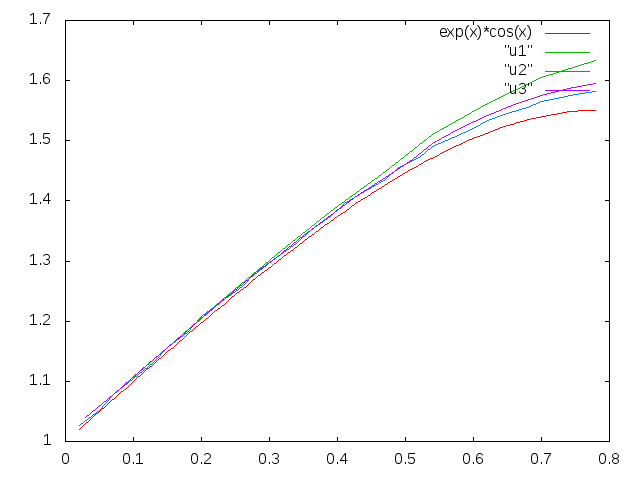
\includegraphics[scale=0.65]{img/graphic.png}
\label{figura1}
\caption{Aproximación para 25, 50 y 100 nodos} 
\end{figure}

A continuación usaremos de nuevo el método de Euler para sistemas, pero esta vez para tamaños de paso menores, de forma que podamos ver la evolución del error según el número de nodos usado. Tras las ejecuciones los datos obtenidos son los siguientes:

    \begin{table}[H]
        \centering
        \setlength\extrarowheight{3pt}
        
        \begin{tabular}{|c|c|c|c|c}
            \hline
            \textbf{h} & {\textbf{u($\pi$/4)}} & \textbf{Error} \\ 
            \hline
                120 & 1.581351427438043 & 0.030468230520017\\
            \hline
                240 & 1.566883575533628 & 0.016000378615602\\
            \hline
                360 & 1.561353411976403 & 0.010470215058378\\
            \hline
                480 & 1.558765635465628 & 0.007882438547603\\
            \hline
                600 & 1.557203467884946 & 0.0063202709669205\\
            \hline
                720 &  1.556204299202344 & 0.0053211022843184\\
            \hline
                840 & 1.555409383683734 & 0.0045261867657087\\
            \hline
        \end{tabular}
        
        \caption{Descripción del actor restaurante.}
        \label{table:actor:restaurante}             
    \end{table}


\section{Artículo}

En esta sección realizaremos un resumen del artículo ``Numerical solution of differential equations using multiquadric radial basis function networks"(Nam Mai-Duy, Thanh Tran-Cong; 2001). En este artículo se introducirá una técnica novedosa para la resolución de ecuaciones diferenciales ordinarias, a partir de ahora ODEs, y ecuaciones diferenciales parciales, PDEs. Previo al resumen veamos una breve descripción de red neuronal:\\

En el contexto de la informática una red neuronal es un conjunto de unidades menores llamadas neuronas interconectadas entre sí. Cada neurona, a partir de un conjunto de entradas, es capaz de proporcionar una salida en la que aparentemente se aplica inteligencia. Para generar dicha salida se hace uso de funciones con carácter probabilísticos cuyos pesos habrá que ajustar en la fase de entrenamiento. Esta fase de entrenamiento consistene en proporcionar un conjunto de entradas con sus correspondientes salidas, de forma que la red neuronal se ajusta según estos datos proporcionados, es decir, modifica dichas funciones a través del conocimiento proporcionado y de esta forma ``aprende" a dar la respuesta correcta para el problema en cuestión con una probabilidad de acierto muy elevada.\\

Los métodos clásicos para la obtención de aproximaciones de la solución de ecuaciones diferenciales suponen un proceso costoso al tener que seleccionar un dominio adecuado con un número finito de elementos para proceder con el mismo. En este artículo, como ya se ha comentado, se presenta un método novedoso para la resolución de ecuaciones diferenciales lineales haciendo uso de redes neuronales artificiales en el que no habrá problema para seleccionar el dominio. \\

En el método presentado en el artículo se hace uso de redes de base radial, que son redes neuronales en las que las funciones que determinan la salida serán funciones de base radial, esto es, funciones reales cuya imagen para cada punto viene determinada por la distancia al origen, es decir, diremos que $\phi:\mathbb{R}^n\to \mathbb{R} $  es radial si

$$\exists \Phi:\mathbb{R}\to \mathbb{R}\ \ tq\ \phi(x)=\Phi(\parallel x\parallel)\ \ \forall x\in\mathbb{R}^n$$

Existen diversas funciones de base radial, pero los autores harán uso de las funciones multicuadráticas, que son aquellas que se definen como sigue:

$$\phi(r) = \sqrt{\epsilon^2+r^2}$$

Notaremos a los métodos numéricos que hacen uso de las redes neuronales con funciones de base radial como RBFN, y podremos clasificarlas como directos (DRBFN) e indirectos (IRBFN). Recordemos en primer lugar que los métodos numéricos directos para la aproximación de funciones y sus derivadas son aquellos que aproximan la función y la aproximación de las sucesivas derivadas serán las sucesivas derivadas de dicha aproximación, mientras que los métodos indirectos son aquellos en los que en primer lugar se aproximan las derivadas de mayor orden y posteriormente se consiguen las de orden menor integrando dicha aproximación. Puesto que se hace uso de funciones multicuadráticas, la función aproximación será de la forma:

$$ u(x) = \sum\limits_{i=1}^{m} w^{(i)}g^{(i)}(x) = \sum\limits_{i=1}^{m} w^{(i)}\sqrt{\epsilon^{(i)^2}+x^2}$$

Donde m es el número de neuronas utilizadas en el método y $w^{(i)}$ los pesos asociados a cada neurona obtenidos durante la fase de entrenamiento. Más adelante veremos como determinar $\epsilon^{(i)}$. La norma del error que se cometerá vendrá determinada por:

$$N_e = \sqrt{\frac{\sum\limits_{i=1}^{m}(u_e(x^{(i)})-u(x^{(i)}))^2}{\sum\limits_{i=1}^{m}u_e(x^{(i)})^2}}$$

Para aplicar el método debemos contar con la imagen de una serie de puntos de colocación o nodos $\{u(x^{(i)})=y^{(i)}\}_{i=1}^{n}$ que servirán como entrenamiento para la determinación de la función. Se contará además con otro tipo de puntos, que llamaremos centros, y que se repartirán uniformemente en forma de malla a lo largo de todo el dominio de la función a aproximar. En la figura 1 podemos ver la distribución de los centros y los nodos.\\

\begin{figure}
\centering
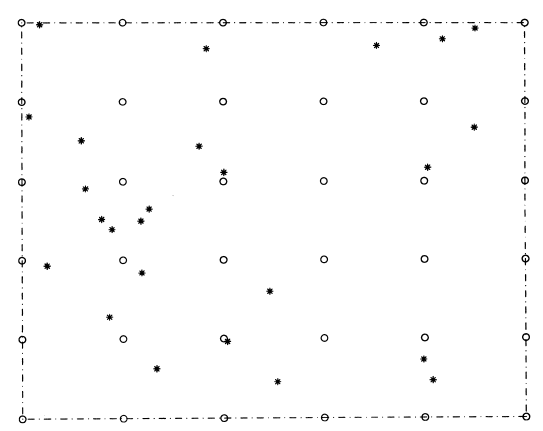
\includegraphics[scale=0.45]{img/centros}
\label{figura1}
\caption{Distribución de los centros ($\circ$) y nodos ($\bullet$)} 
\end{figure}

A lo largo del artículo los autores darán resultados de la aplicación del método para la resolución de ODEs en dominios regulares y de PDEs en elipses. Entenderemos por dominio regular a aquel que esté formado por el producto cartesiano de intervalos. En dichos dominios nos será relativamente fácil establecer los centros, y aquí es donde reside la única libertad que podemos aplicar en el método. Veamos por qué.\\

A la hora de crear la malla en nuestro dominio podremos hacerla más densa o menos con total libertad, pero estableceremos la siguiente relación con $\epsilon^{(i)}$:
$$\epsilon^{(i)} = \beta d^{(i)}$$

Donde $d^{(i)}$ es la distancia del i-ésimo centro al centro más cercano. Podremos elegir $\beta > 0$ con libertad, aunque dicho parámetro influirá en la función aproximación obtenida. Aunque no hay forma conocida de determinar el valor óptimo de $\beta$ en cada ocasión, experimentalmente los autores han obtenido que los valores óptimos suelen centrarse en el intervalo [7,10].\\

A continuación se pasa al estudio de la aplicación del método para PDEs en dominios elípticos. El problema que surge en este momento es la generación de la malla. La solución es simple: si $\Omega$ es nuestro dominio elíptico, tomaremos $\Omega^*$ dominio regular tal que $\Omega^*\supset \Omega$ , y aplicaremos el método para el dominio $\Omega^*$, aunque los nodos se encontrarán todos dentro de $\Omega$.\\

Tras una serie de ejemplos los autores muestran como el método IRBFN consigue resultados más adecuados que los conseguidos con el método directo, y además, los resultados son mejores para un mayor rango de $\beta$. Los autores dicen no tener una demostración teórica que corrobore este hecho, pero dan la idea intuitiva del porqué de este hecho: al cometer un error determinado con el método directo, al derivar para obtener las sucesivas derivadas intensificamos el error, mientras que en el método indirecto disminuimos el efecto del error cometido.\\%Distribución del error

Durante el artículo también se realizan comparaciones con los métodos clásicos y se concluye que el método directo, en términos de error, es igual de adecuado que los métodos clásicos, mientras que el método indirecto consigue resultados de varios órdenes de magnitud mayor.\\

Finalmente se habla de una futura adecuación del método para dominios irregulares construyendo un recubrimiento finito de dominios regulares y procediendo de igual forma que con el caso del dominio elíptico.\\


\end{document}
